%PREAMBULO MEMORIA
\documentclass[a4paper, 12pt]{book}
\usepackage[a4paper, left=2.5cm, right=2.5cm, top=2cm, bottom=3cm]{geometry}
\usepackage[utf8]{inputenc} %Para introducir tildes
\usepackage{url} %Para introducir urls
\usepackage{tocbibind} %Bibliografía en el indice
\usepackage[spanish]{babel}
\usepackage[toc]{blindtext}
\usepackage{tocbibind}
\usepackage{float} %Para posicionar figuras
\usepackage{graphicx}
\usepackage{fancyhdr}
\usepackage{hyperref}
\usepackage{subfig} %Para insertar varias figuras
\usepackage{titlesec, blindtext, color}
%%Estilo de fuente
\usepackage{lmodern}
\usepackage[OT1]{fontenc}
% Personalización de Formato de Capítulo
\usepackage[Lenny]{fncychap}
%Declaración de lenguaje HTML5 para paquete listings
\usepackage{color}
\definecolor{lightgray}{rgb}{0.95, 0.95, 0.95}
\definecolor{darkgray}{rgb}{0.4, 0.4, 0.4}
\definecolor{purple}{rgb}{0.65, 0.12, 0.82}
\definecolor{editorGray}{rgb}{0.95, 0.95, 0.95}
\definecolor{editorOcher}{rgb}{1, 0.5, 0} % #FF7F00 -> rgb(239, 169, 0)
\definecolor{editorGreen}{rgb}{0, 0.5, 0} % #007C00 -> rgb(0, 124, 0)
\definecolor{orange}{rgb}{1,0.45,0.13}		
\definecolor{olive}{rgb}{0.17,0.59,0.20}
\definecolor{brown}{rgb}{0.69,0.31,0.31}
\definecolor{purple}{rgb}{0.38,0.18,0.81}
\definecolor{lightblue}{rgb}{0.1,0.57,0.7}
\definecolor{lightred}{rgb}{1,0.4,0.5}
\usepackage{upquote}
\usepackage{listings}
\lstset{backgroundcolor=\color{editorGray}}
% CSS
\lstdefinelanguage{CSS}{
  keywords={color,background-image:,margin,padding,font,weight,display,position,top,left,right,bottom,list,style,border,size,white,space,min,width, transition:, transform:, transition-property, transition-duration, transition-timing-function},	
  sensitive=true,
  morecomment=[l]{//},
  morecomment=[s]{/*}{*/},
  morestring=[b]',
  morestring=[b]",
  alsoletter={:},
  alsodigit={-}
}

% JavaScript
\lstdefinelanguage{JavaScript}{
  morekeywords={typeof, new, true, false, catch, function, return, null, catch, switch, var, if, in, while, do, else, case, break},
  morecomment=[s]{/*}{*/},
  morecomment=[l]//,
  morestring=[b]",
  morestring=[b]'
}

\lstdefinelanguage{HTML5}{
  language=html,
  sensitive=true,	
  alsoletter={<>=-},	
  morecomment=[s]{<!-}{-->},
  tag=[s],
  otherkeywords={
  % General
  >,
  % Standard tags
	<!DOCTYPE,
  </html, <html, <head, <title, </title, <style, </style, <link, </head, <meta, />, <footer, </footer,
	% body
	</body, <body,
	% Divs
	</div, <div, </div>, <section, </section
	% Paragraphs
	</p, <p, </p>,
	% scripts
	</script, <script,
  % More tags...
  <canvas, /canvas>, <svg, <rect, <animateTransform, </rect>, </svg>, <video, <source, <iframe, </iframe>, </video>, <image, </image>, <header, </header, <article, </article, </nav, <nav, <h1, </h1
  },
  ndkeywords={
  % General
  =,
  % HTML attributes
  charset=, src=, id=, width=, height=, style=, type=, rel=, href=,
  % SVG attributes
  fill=, attributeName=, begin=, dur=, from=, to=, poster=, controls=, x=, y=, repeatCount=, xlink:href=,
  % properties
  margin:, padding:, background-image:, border:, top:, left:, position:, width:, height:, margin-top:, margin-bottom:, font-size:, line-height:,
	% CSS3 properties
  transform:, -moz-transform:, -webkit-transform:,
  animation:, -webkit-animation:,
  transition:,  transition-duration:, transition-property:, transition-timing-function:,
  }
}

\lstdefinestyle{htmlcssjs} {%
  % General design
%  backgroundcolor=\color{editorGray},
  basicstyle={\footnotesize\ttfamily},   
  frame=b,
  % line-numbers
  xleftmargin={0.75cm},
  numbers=left,
  stepnumber=1,
  firstnumber=1,
  numberfirstline=true,	
  % Code design
  identifierstyle=\color{black},
  keywordstyle=\color{blue}\bfseries,
  ndkeywordstyle=\color{editorGreen}\bfseries,
  stringstyle=\color{editorOcher}\ttfamily,
  commentstyle=\color{brown}\ttfamily,
  basicstyle=\footnotesize\fontfamily{fvm}\selectfont, % use Bera    Mono  
  % Code
  language=HTML5,
  alsolanguage=JavaScript,
  alsodigit={.:;},	
  tabsize=2,
  showtabs=false,
  showspaces=false,
  showstringspaces=false,
  extendedchars=true,
  breaklines=true,
  % German umlauts
  literate=%
  {Ö}{{\"O}}1
  {Ä}{{\"A}}1
  {Ü}{{\"U}}1
  {ß}{{\ss}}1
  {ü}{{\"u}}1
  {ä}{{\"a}}1
  {ö}{{\"o}}1
}
%

\title{Memoria del Proyecto}
\author{Javier Fernández Morata}

\renewcommand{\baselinestretch}{1.5}

\begin{document}

\renewcommand{\refname}{Bibliografía}
%%%%%%%%%%%%%%%%%%%%%%%%%%%%%%%%%%%%%%%%%%%%%%%%%%%%%%%%%%%%%%%%%%%%%%%%%%%%%%%
% PORTADA
%%%%%%%%%%%%%%%%%%%%%%%%%%%%%%%%%%%%%%%%%%%%%%%%%%%%%%%%%%%%%%%%%%%%%%%%%%%%%%%
\begin{titlepage}
\begin{center}
\begin{tabular}[c]{c c}
\includegraphics[scale=0.25]{img/logo_vect.png} &
\begin{tabular}[b]{l}
\Huge
\textsf{UNIVERSIDAD} \\
\Huge
\textsf{REY JUAN CARLOS} \\
\end{tabular}
\\
\end{tabular}

\vspace{3cm}
\Large
INGENIERÍA EN TECNOLOGÍAS DE LA TELECOMUNICACIÓN

\vspace{0.4cm}
\Large
Curso Acádemico 2018/2019

\vspace{0.8cm}
Trabajo Fin de Grado

\vspace{2.5cm}
\Large
PYCARDIO: PAQUETE PARA ANÁLISIS DE SEÑALES CARDIACAS

\vspace{4cm}
\large
Autor : Javier Fern\'andez Morata \\
Tutor : Dr. Felipe Ortega
\end{center}
\end{titlepage}

\newpage
\thispagestyle{empty}
%%%%%%%%%%%%%%%%%%%%%%%%%%%%%%%%%%%%%%%%%%%%%%%%%%%%%%%%%%%%%%%%%%%%%%%%%%%%%%%
% PARA FIRMAR
%%%%%%%%%%%%%%%%%%%%%%%%%%%%%%%%%%%%%%%%%%%%%%%%%%%%%%%%%%%%%%%%%%%%%%%%%%%%%%%
\clearpage
\pagenumbering{gobble}
\chapter*{}

\vspace{-4cm}
\begin{center}
  \large
  \textbf{Trabajo Fin de Grado}

  \vspace{1cm}
  \large
  \{\{Título del Trabjo con Letras Capitales para Sustantivos y Adjetivos\}\}

  \vspace{1cm}
  \large
  \textbf{Autor :} Javier Fernández Morata \\
  \textbf{Tutor :} Dr. Felipe Ortega
\end{center}

\vspace{1cm}
La defensa del presente Proyecto Fin de Carrera se realiza el día \qquad$\;\,$ de \qquad\qquad\qquad\qquad \newline de 20XX, siendo calificada por el siguiente tribunal:

\vspace{0.5cm}
\textbf{Presidente:}

\vspace{1.2cm}
\textbf{Secretario:}

\vspace{1.2cm}
\textbf{Vocal:}

\vspace{1.2cm}
y habiendo obtenido la siguiente calificación:

\vspace{1cm}
\textbf{Calificación:}

\vspace{1cm}
\begin{flushright} Fuenlabrada, a \qquad$\;\,$ de
  \qquad\qquad\qquad\qquad de 20XX
\end{flushright}


%%%%%%%%%%%%%%%%%%%%%%%%%%%%%%%%%%%%%%%%%%%%%%%%%%%%%%%%%%%%%%%%%%%%%%%%%%%%%%%
% DEDICATORIA
%%%%%%%%%%%%%%%%%%%%%%%%%%%%%%%%%%%%%%%%%%%%%%%%%%%%%%%%%%%%%%%%%%%%%%%%%%%%%%%
\chapter*{}
\begin{flushright}
  \textit{\_Escribimos Dedicatoria\_}
\end{flushright}


%%%%%%%%%%%%%%%%%%%%%%%%%%%%%%%%%%%%%%%%%%%%%%%%%%%%%%%%%%%%%%%%%%%%%%%%%%%%%%%
% AGRADECIMIENTOS
%%%%%%%%%%%%%%%%%%%%%%%%%%%%%%%%%%%%%%%%%%%%%%%%%%%%%%%%%%%%%%%%%%%%%%%%%%%%%%%
\chapter*{Agradecimientos}

[ AQUÍ VAN LOS AGRADECIMIENTOS ]

%%%%%%%%%%%%%%%%%%%%%%%%%%%%%%%%%%%%%%%%%%%%%%%%%%%%%%%%%%%%%%%%%%%%%%%%%%%%%%%
% RESUMEN
%%%%%%%%%%%%%%%%%%%%%%%%%%%%%%%%%%%%%%%%%%%%%%%%%%%%%%%%%%%%%%%%%%%%%%%%%%%%%%%
\chapter*{Resumen}

Aquí viene un resumen del proyecto.Ha de constar de tres o cuatro párrafors, donde se presente de manera clara y concisa de qué va el proyecto.
Han de quedar respondidas las siguientes preguntas:
\begin{itemize}
  \item ¿De qué va este proyecto? ¿Cuál es el objetivo principal?
  \item ¿Cómo se ha realizado? ¿Qué tecnologías están involucradas?
  \item ¿En qué contexto se ha realizado el Proyecto? Es un proyecto dentro de un marco general?
\end{itemize}

 %%%%%%%%%%%%%%%%%%%%%%%%%%%%%%%%%%%%%%%%%%%%%%%%%%%%%%%%%%%%%%%%%%%%%%%%%%%%%%%
 % ÍNDICE
 %%%%%%%%%%%%%%%%%%%%%%%%%%%%%%%%%%%%%%%%%%%%%%%%%%%%%%%%%%%%%%%%%%%%%%%%%%%%%%%
%% contenidos
\tableofcontents

%%%%%%%%%%%%%%%%%%%%%%%%%%%%%%%%%%%%%%%%%%%%%%%%%%%%%%%%%%%%%%%%%%%%%%%%%%%%%%%
% CAPÍTULO 1 - INTRODUCCIÓN Y OBJETIVOS
%%%%%%%%%%%%%%%%%%%%%%%%%%%%%%%%%%%%%%%%%%%%%%%%%%%%%%%%%%%%%%%%%%%%%%%%%%%%%%%

\chapter{Introducción y objetivos}
\label{chap:intro}
\pagenumbering{arabic}
En este proyecto tratamos la importancia de seguir unas buenas pautas para la gestión y distribución de código. Donde de todas ellas ahondaremos en la creación de documentación web, donde nos ayudaremos de varias tecnologías. \\
El objetivo por tanto de este proyecto, es presentar las pautas a seguir para facilitar las contribuciones futuras en proyectos de software libre y mostrar una de ellas como, la documentación. \\
Por tanto, la intención de este capítulo es mostrar el contexto, la motivación que  me ha llevado para realizar dicho proyecto, objetivos de este, y la estructura que vamos a seguir para mostrar lo realizado.

\section{Contexto}
\label{sec:contex}
A los largos de los años, el software ha pasado por varias etapas en cuanto a su privatización. Antes del \emph{boom} de la informática, los que hacían uso de ella, compartían \emph{software} sin ninguna restricción, pero cuando llegaron los años 80 las compañías que vendían las computadoras comercializaban estas usando sistemas operativos privados, forzando al usuario a aceptar restricciones legales de modificar dicho \emph{software}.\\ 
Por estos años y debido a un error con un dispositivo, Richard Stallman fundó el proyecto GNU e introdujo la definición de \emph{software libre}. ¿Qué es software libre? Software libre es la cuestión de libertad de ejecutar, copiar, distribuir, estudiar, cambiar y mejorar el software.
\newpage
Es decir, significa que los usuarios de dicho software disponemos de las cuatro libertades esenciales: 
\begin{itemize}
    \item Libertad 0, libertad para ejecutar el \emph{software} con cualquier propósito
    \item Libertad 1, acceso al código fuente; por lo que podemos modificar dicho \emph{software} para hacer lo que el usuario quiera
    \item Libertad 2, redistribuir copias 
    \item Libertad 3, redistribución de versiones modificadas.
\end{itemize}

Y por tanto, uno de los objetivos de este proyecto es facilitar las contribuciones futuras para unos módulos sobre ingeniería biomédica desarrollados en la Universidad Rey Juan Carlos I, donde para ello, se creara una documentación web, usando tecnologías como Jekyll, que es un generador de contenido estático, o herramientas como ReadTheDocs o Sphinx, que facilitan la creación de documentación de \emph{software} 


\section{Motivación Personal}
\label{sec:mot}
Desde que empecé el instituto siempre me he decantado por una manera de trabajar más práctica que teórica. Si algo tengo que destacar de la carrera es el descubrir la programación, algo que sabía que era, pero que nunca había practicado, es decir, no había programado nunca un "Hola Mundo". \\
Una de las asignaturas que más me entusiasmo cursar, fue la de \emph{"Servicios y Aplicaciones Telemáticas"}, en la que desarrollamos aplicaciones web a través del \emph{framework} Django. En este proyecto además de un desarrollo web, con distintas tecnologías que utilice en dicha asignatura, hay otro objetivo, que es el más interesante para mi, que es seguir unas pautas de escribir código para proyectos de \emph{Software libre}.

\section{Objetivos}
\label{sec:objetivos}
El objetivo principal, por tanto, es la creación de un sitio web, para dar a conocer la librería python \emph{pyCardio}. Dicha librería ha sido desarrollada por varios alumnos y profesores de esta Universidad. Donde con esta web lo que se propone es dar a conocer los módulos de la librería y mostrar su documentación. \\
Otro propósito de dicha web, al ser un proyecto de \emph{Software libre}, es facilitar la contribución al código de este paquete. Para alcanzar dichos fines, han sido abordados las siguientes metas secundarias :
\begin{itemize}
    \item Aprendizaje de nuevas tecnologías usadas en el proyecto.
    \item Publicar contenido mediante Jekyll 
    \item Crear la docWeb en GitHub Pages
    \item Aprender a usar Liquid, para optimizar el desarrollo del contenido
\end{itemize}

\section{Estructura de la memoria}
\label{sec:estruc}
Para finalizar la introducción, se explica como va a ir estructurada la memoria seguida de un breve resumen del contenido que trata cada sección: 
\begin{enumerate}
    \item En el capítulo uno, como ya hemos visto, se introduce el por qué de este proyecto así como los objetivos que se tratan en él.
    \item En el segundo, \emph{Soluciones tecnológicas}, se explican las tecnologías usadas en el proyecto tanto en la generación del sitio web, como de gestión y documentación de proyectos Python.
    \item En el tercer capítulo, \emph{Gestión de código}, trataremos sobre la gestión de código en python y sobre el paquete que centramos el objetivo de este proyecto \emph{pyCardio}.
    \item En este cuarto capítulo, \emph{Propuesta del diseño web del proyecto}, presentamos la web del proyecto donde se incluirá la documentación del módulo, guía de instalación, así como una guía para futuras contribuciones.
    \item En el quinto y último capítulo, \emph{Conclusiones y trabajo futuro}, exponemos las conclusiones sacadas así como el trabajo que se debería realizar tras la finalización de este mismo.
\end{enumerate}

%%%%%%%%%%%%%%%%%%%%%%%%%%%%%%%%%%%%%%%%%%%%%%%%%%%%%%%%%%%%%%%%%%%%%%%%%%%%%%%
% CAPÍTULO 2 - ARQUITECTURA GENERAL
%%%%%%%%%%%%%%%%%%%%%%%%%%%%%%%%%%%%%%%%%%%%%%%%%%%%%%%%%%%%%%%%%%%%%%%%%%%%%%%
\chapter{Soluciones tecnológicas}
\label{chap:Arqui}
Este capítulo constará de dos partes. Una primera donde se muestra una visión general de las tecnologías que usaremos para la creación de la página web, y una segunda donde explicamos brevemente cada tecnología utilizada.

    %%
    % 2.1 - ARQUITECTURA
    %%
\section{Arquitectura general}
\label{sec:arqui}
En cualquier proyecto de desarrollo web existen dos tipos de tecnologías, BackEnd y FrontEnd. Por tanto, antes de exponer la visión general de nuestra web. ¿Qué significan estos dos términos?:
\begin{itemize}
    \item \textbf{BackEnd:} Tecnologías que trabajan en el lado del servidor,es decir, tecnologías en toma de datos, procesarlos, envío al usuario. Sin estas, las tecnologías del \emph{frontEnd} no tendrían nada que mostrar.
    \item \textbf{FrontEnd:} Tal y como hemos comentado, son las tecnologías que se encargan de mostrar el contenido, es decir, tecnologías centradas en el lado de la aplicación como CSS, HTML5, JavaScript.
\end{itemize}
Una vez diferenciada estas capas, en nuestro \emph{BackEnd} podemos diferencias tecnología donde se alojara tanto nuestro contenido web como nuestro código fuente en \emph{GitHub}, tecnología que además proporcionará otras como soporte de problemas (ITS), tecnologías sobre cobertura de código. \\
\begin{figure}[h]
    \centering
    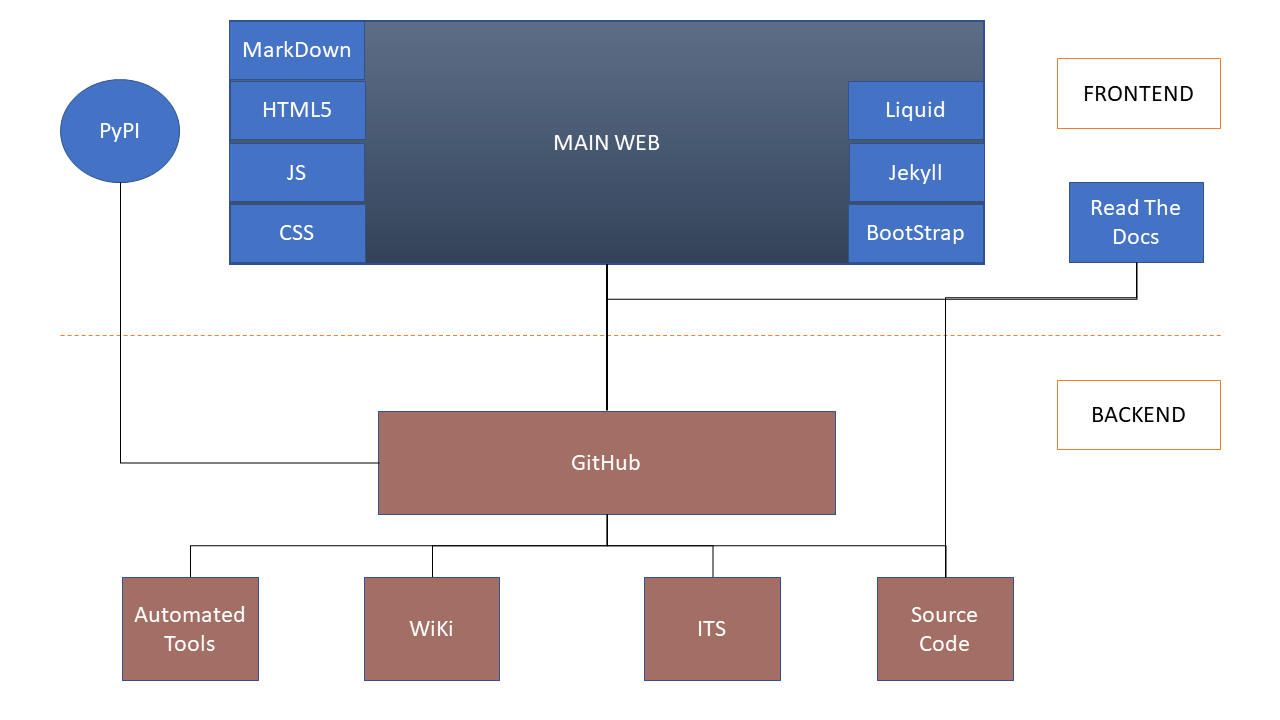
\includegraphics[width=\textwidth]{img/arqui_general.png}
    \caption{Arquitectura General de la Web}
    \label{fig:arquiGeneral}
\end{figure}
En la capa \emph{FrontEnd} observamos como todas las tecnologías que colaborarán son aquellas ya conocidascomo HTML5, CSS; donde cuyo objetivo es mostrar contenido y otras nuevas como \emph{Jekyll}. Observando la figura \ref{fig:arquiGeneral} vemos que otras dos tecnologías nos apoyarán en mostrar el funcionamiento del módulo \emph{PyCardio}, una para mostrar la documentación de los módulos(\emph{ReadTheDocs}) y otra donde también se alojará el código fuente siendo así una aplicación de terceros de Python(PyPI).
    
    %%
    % 2.2 - BackEnd
    %%
\section{BackEnd}
\label{sec:backend}
        %%
        % 2.2.1 - CONTROL DE VERSIONES CON GIT. GITHUB
        %%
\subsection{Control de versiones con Git. GitHub}
\label{subsec:git}
\begin{figure}[h]
    \centering
    \subfloat{
        
\includegraphics[scale=0.7]{img/logo_git.png}
        \label{img:logoGit}
    } \hspace{30mm}
    \subfloat{
        
\includegraphics{img/logo_github.png}
        \label{img:logoGithub}
    }
\end{figure}
Este proyecto al ser un trabajo de \emph{software libre}, significa que el código sufrirá cambios de distintos autores, por lo que es necesario un sistema de control de versiones. Para que un sistema sea de control de versiones debe proporcionar un mecanismo de almacenamiento de los elementos que se desea gestionar, posibilidad de realizar cambios sobre los elementos almacenados y un registro histórico de las acciones realizadas con cada elemento o conjunto de elementos. \\
El sistema que se ha escogido debido a nuestra arquitectura de almacenamiento de código y por su seguridad, comodidad y velocidad, es \emph{Git}. Una gran diferencia de \emph{Git} respecto a los demás sistemas de control de versiones es la manera de llevar el registro de cambios sobre sus datos, mientras que la mayoría de sistemas almacenan la información como una lista de cambios, en \emph{Git}, cada vez que se realiza un cambio sobre un archivo \emph{Git} hace una instantánea, y guarda una referencia sobre el archivo sin estos cambios. Para ser mas eficiente, si los archivos no han sido modificados, \emph{Git} no almacena el archivo de nuevo. Esta distinción influye en uno de los mayores beneficios de \emph{Git}, las ramificaciones, tema que trataremos a continuación, viendo como trabajar en un proyecto siguiendo una serie de reglas impuestas por \emph{GitFlow}. \\
\textbf{¿Cómo funciona \emph{Git}?}\\
Todo el funcionamiento de este sistema de control de versiones es mayoritariamente local, es decir, no se necesita información de ningún servidor haciendo así que este sistema sea muy rápido respecto a otros que necesitan información remota para sus operaciones. \\
\emph{Git} tiene tres estados para los archivos que trabajamos:
\begin{itemize}
    \item \textbf{Committed}: Este estado indica que los archivos que han sido modificados, se han almacenado de manera segura en la base de datos local.
    \item \textbf{Modified}: Indica que los archivos que han sido modificados, no han sido confirmados, es decir, los archivos no se han almacenado de forma segura en la base de datos local.
    \item \textbf{Staged}: Estado que marca archivos modificados para la siguiente confirmación. 
\end{itemize}
Estos tres estados nos lleva a diferenciar las siguientes áreas de trabajo: 
\begin{figure}[ht]
    \centering
    \label{fig:gitStates}
    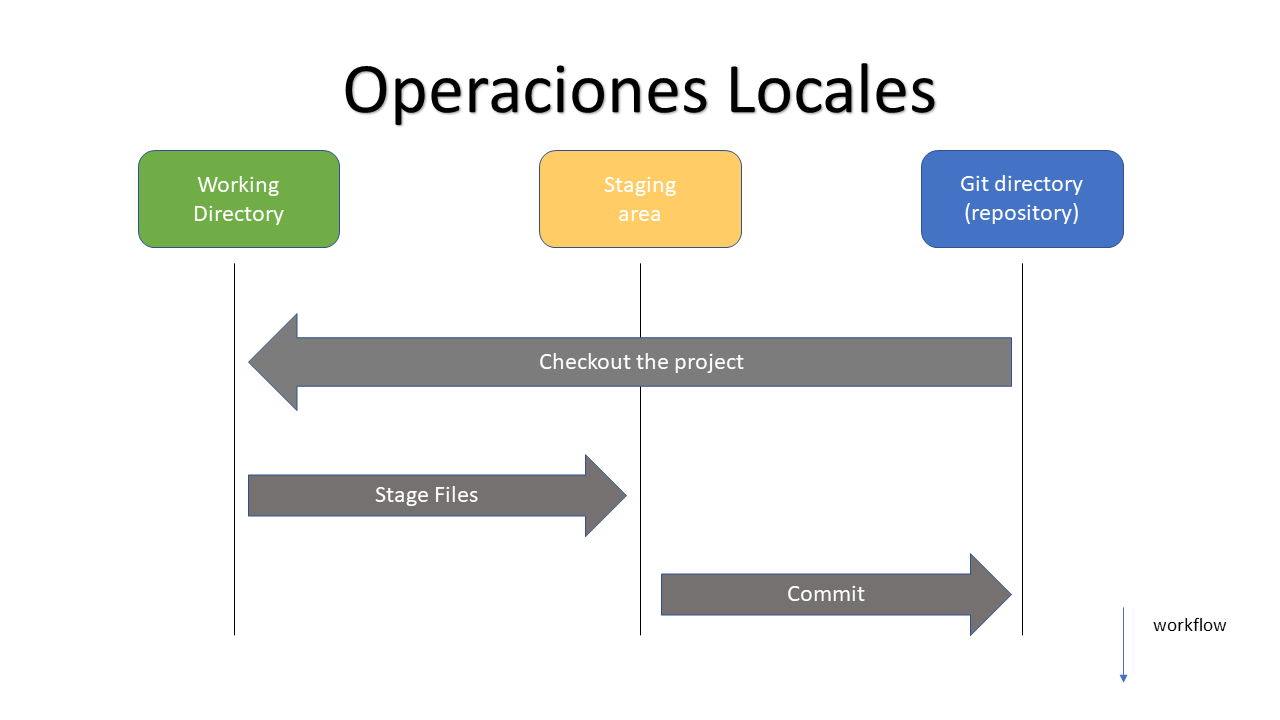
\includegraphics[width=\textwidth]{img/git_states.png}
    \caption{ Esquema de los estados de un repositorio Git}
\end{figure}
\begin{itemize}
    \item \textbf{Working Directory}: Este área es donde obtenemos la copia del proyecto, lista para usarse o modificarse, sin influir en la copia original.
    \item \textbf{Staged Area}: Área en la que se recoge los cambios que van a realizarse sobre los archivos antes de confirmarse.
    \item \textbf{Git Directory}: Estado de los archivos originales del proyecto, incluidos metadatos. Cuando se confirma un archivo, \emph{Git} toma los cambios del área de preparación (Staged Área) y almacena los cambios nuevos en el directorio \emph{Git}.
\end{itemize}
Por tanto, el flujo que hay que seguir para trabajar con este sistema de control de versiones es el representado en la figura \ref{fig:gitStates}, donde como vemos tras modificar una serie de archivos en el directorio de trabajo preparamos los archivos añadiéndolos al staged area, se confirman los cambios realizados sobre estos, añadiendo así las instantáneas (copias de los archivos con los cambios confirmados) en el directorio \emph{Git}. 

Una vez que hemos visto como trabaja \emph{Git} nos queda responder la pregunta de \textit{¿Qué es GitHub?} \emph{GitHub} es una plataforma de desarrollo colaborativo de software para alojar proyectos utilizando los mencionados repositorios \emph{Git}, es decir, aloja el código en la nube y brinda herramientas para el trabajo de equipo en el proyecto. Otra de las características de \emph{GitHub} es el poder contribuir en el desarrollo de software de los demás, algo esencial en cualquier proyecto de software libre. \textit{¿Qué herramientas proporciona para el trabajo en equipo?} \emph{GitHub} proporciona un amplio abanico de funcionalidades , entre ellas, destaca una wiki para el mantenimiento de las versiones de las paǵinas, un sistema de seguimiento de problemas permitiendo al equipo detallar los problemas con lo desarrollado y una herramienta de revisión de código. \\ 
Antes de dar por finalizada la sección sobre \emph{Git}, debemos hablar sobre \emph{GitFlow}, extensión de \emph{GitHub} que permite un mantenimiento y estrategia para las ramificicaciones en un proyecto de desarrollo. Esta estrategia y mantenimiento se basa en una serie de reglas, donde se destacan dos ramas principales: rama \textit{master}, y rama \textit{develop}.La \textit{master} se usa cada vez que tengamos código para producción y la rama \textit{develop} para el código que conformará la nueva versión del proyecto \\
\begin{figure}[H]
    \centering
    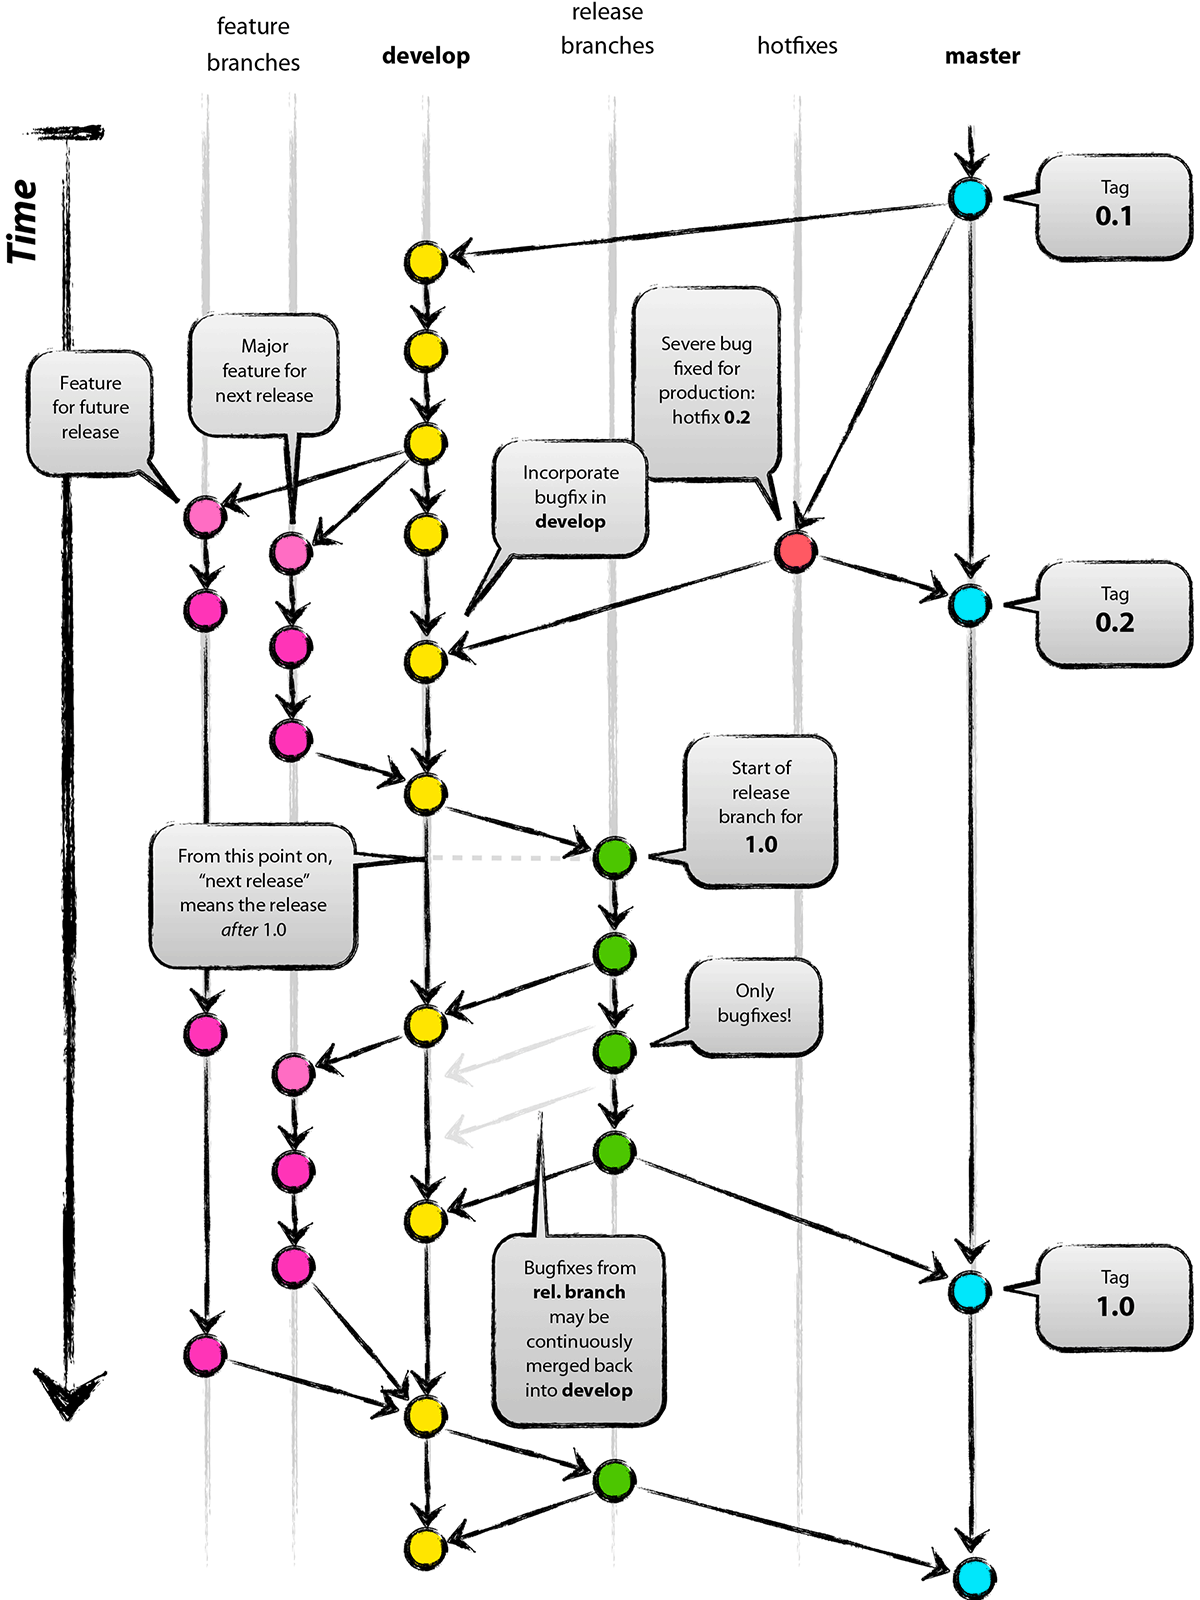
\includegraphics[scale=0.2]{img/git_flow.png}
    \caption{WorkFlow impuesto por la estrategia y mantenimiento de \emph{GitFlow}}
    \label{fig:gitFlow}
\end{figure}
Por tanto, cada vez que se incorpora código a la rama \textit{master}, tenemos nueva versión. A parte de las ramas principales, observando la figura \ref{fig:gitFlow} podemos distinguir tres tipos de ramas auxiliares, donde cada una sigue sus propias reglas:
\begin{itemize}
    \item \textbf{Feature:} Se originan a partir de la rama \textit{develop}, y  se utilizan para incorporar nuevas características a la aplicación.
    \item \textbf{Release:} Rama que se crea al igual que \textit{feature}, a partir de la rama \textit{develop}. En ellas se depura el código el cual se va a pasar a la producción, es decir, a la rama \textit{master}. 
    \item \textbf{Hotfix:} Rama cuyo objetivo es parecido al de la rama \textit{feature}, pero esta se origina a partir de la \emph{master}, y los errores que corregimos en esta rama no están planificados a diferencia de la rama \emph{feature}, que sí lo están. 
\end{itemize}
De esta manera el uso que daremos de \emph{GitHub} es el de construir un repositorio donde alojaremos el código de nuestro paquete, permitiendo así que cualquiera pueda aportar ideas al proyecto o mejorar el software.
        
        %%
        % 2.2.2 - Issue Tracking System
        %%
\subsection{ITS (Issue Tracking System)}
\label{subsec:issue}
\emph{GitHub} proporciona un sistema de seguimiento de incidentes (en inglés \textit{issue tracking system}, funcionalidad que permite administrar y mantener una lista de incidentes, al tratar de \emph{software}, una incidencia será una solicitud de modificación, corrección o mejora
    %%
    % 2.3 - FRONTEND
    %%F
\section{FrontEnd}
\label{sec:frontEnd}
        %%
        % 2.3.1 - GITHUB PAGES & Jekyll
        %%
\subsection{GitHub Pages y Jekyll}
\label{subsec:githubJekyll}
\emph{GitHub Pages} y \emph{Jekyll} se usan conjuntamente para generar sitios web estáticos , donde \emph{Jekyll} se encarga de generar los sitios web y \emph{GitHub Pages} de servicio de alojamiento. Ambos servicios están integrados. Para explicar como trabajan ambos servicios, vamos a tratarlos primero por separado.

\subsection*{GitHub Pages}
\label{subsec:githubpages}
Es un servicio de alojamiento web que ofrece \emph{GitHub}, se usa para alojar sitios web estáticos usando directamente un repositorio \emph{Git}. Para aclarar la principal ventaja de \emph{GitHub Pages} frente a otros servidores vamos a definir que es una pagina web estática y que se diferencia respecto a una página web dinámica. \\
\textbf{¿Qué es una página web estática?}\\
Una página web estática es aquel documento web que muestra el mismo contenido para todos los usuarios, es decir, que no es personalizable o no hay elección de interactuar con ella para ordenar, ocultar o modificar contenido (páginas dinámicas). Una de las ventajas principales de este tipo de páginas es lo económico que resulta crearlas, sin tener que usar ningún tipo de programación especial. Estas páginas son útiles para el objetivo de simplemente mostrar contenido. Hay que destacar que la mayor desventaja de generar sitios web estáticos son su actualización haciendo de esta algo tedioso. \\ 
Una vez aclarado, la ventaja principal, a parte de todas las proporcionadas por ser un repositorio \emph{Git}, es que al no necesitar base de datos para servir el contenido, solo se requiere un servidor web que vaya sirviendo el contenido que se solicita.

\subsection*{Jekyll}
\label{subsec:jekyll}
\begin{figure}[h]
    \centering
    
\includegraphics[scale=0.3]{img/logo_jekyll.png}
    \label{img:logoJekyll}
\end{figure}
\emph{Jekyll} es un generador de sitios web estáticos, en vez de trabajar con base de datos, \emph{Jekyll} trabaja con texto plano (MarkDown o Textile) y lenguaje de plantilla (Liquid)  generando la página web. La principal ventaja que podemos inferir de \emph{Jekyll} es que no necesitamos saber HTML, para generar nuestro contenido web, ventaja que contra resta sobre lo tedioso que es tener actualizado un sitio web estático. \\
\begin{figure}[H]
    \centering
    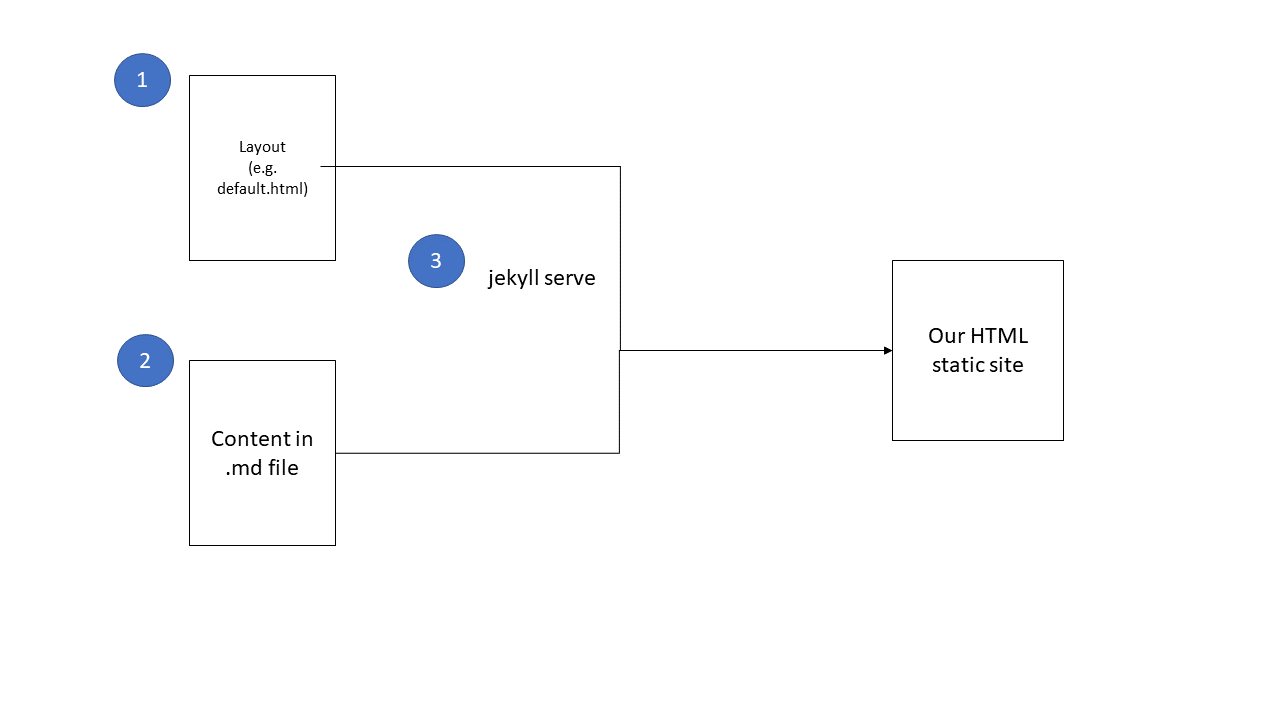
\includegraphics[width=\textwidth]{img/jeyll_process.png}
    \caption{Proceso para web básica con Jekyll}
    \label{fig:jekyllProc}
\end{figure}
Tal y como observamos la figura \ref{fig:jekyllProc} el proceso de trabajo para construir webs con \emph{Jekyll} es:
\begin{enumerate}
    \item Creamos un layout o diseño de nuestra página HTML que incluirá  código del lenguaje de programación \emph{Liquid}.
    \item Escribimos nuestro contenido en texto plano (\emph{MarkDown} o \emph{Textile}) donde tendremos un preámbulo indicando el diseño a utilizar para ese post, así como otras características para nuestro contenido HTML.
    \item Ejecutamos \emph{Jekyll} generando nuestro sitio web estático.
\end{enumerate}

Para entender como funcionan estos tres pasos vamos a tratar cada uno por separado dando un  breve resumen apoyado en ejemplos sencillos. Antes de empezar hay que destacar que cuando ejecutamos \emph{Jekyll} sobre nuestro directorio , cuyo fin será el que contenga los archivos de nuestro sitio web estático, establece una estructura creando en nuestra raíz del proyecto una serie de directorios, cuya función son las siguientes:\\
\begin{itemize}
    \item[] \textbf{\_includes:} En el irán las porciones de código que se repetirán para todos el sitio web (p.ej. footer), se incluirán en nuestro layouts con includes.
    \item[] \textbf{\_layouts:} Directorio que contendrá todas las plantillas creadas para el sitio web.
    \item[] \textbf{\_posts:} Lugar donde irán todos los artículos que iremos escribiendo en texto plano. 
    \item[] \textbf{\_drafts:} En esta carpeta guardaremos los borradores de nuestros artículos, es decir, se utiliza para la prueba de código.
    \item[] \textbf{\_site:} Está se genera no al crear el proyecto \emph{Jekyll}, si no al lanzar el servidor, está contendrá todos los HTML montados así como un \textit{index.html} (archivo principal de un sitio web).
    \item[] \textbf{\_config.yml:} Esto no es un directorio, es una archivo, pero también es generado al crear un proyecto \emph{Jekyll} donde en él encontraremos datos de configuración así como indicaciones de qué directorio obtener los datos.
\end{itemize}
Una vez que tenemos claro a que corresponde cada directorio en nuestro proyecto , tratamos a continucación lo mencionando anteriormente, los pasos  de un proyecto \emph{Jekyll}. \\

\textbf{\large{Diseño de Layout}} \\
Layout es una plantilla donde \emph{Jekyll} incrustará el contenido escrito en texto plano. Tal y como hemos comentado antes, estas plantillas deberán almacenarse en el directorio \texttt{\_layout}. En ellas  haremos uso de nuestro código guardado en \texttt{\_include}, un ejemplo como el de incluir un footer al final de mi plantilla \texttt{default.html} es el siguiente: 

\begin{lstlisting}[style=htmlcssjs,title=default.html]
<!-- default.html -->
<footer>
    {{include footer.html}}
</footer>
\end{lstlisting}
\begin{lstlisting}[style=htmlcssjs,title=footer.html]
<!-- footer.html -->
<p>Posted by: Hege Refsnes</p>
<p>Contact information: <a href="mailto:someone@example.com">
  someone@example.com</a>.</p>
\end{lstlisting}
La herramienta que mas optimiza el trabajo a la hora de elaborar estas plantillas de la que hace uso \emph{Jekyll} es \emph{Liquid}. Este lenguaje que trataremos en el siguiente punto hace uso de variables, donde estas son etiquetas, objetos y filtros. Además cualquier archivo \emph{Jekyll} es accesible mediante variables vía \emph{Liquid}. Estas variables pueden ser el título del sitio web (establecido en \texttt{\_config.yml}). La variable más importante es \texttt{\{\{content\}\}}, ya que en ella es donde \emph{Jekyll} incrustará el contenido escrito en texto plano. Un ejemplo sencillo de un layout sería el siguiente:
\begin{lstlisting}[style=htmlcssjs,title=default.html]
<!doctype html>
<html lang="en">
  <head>
    {{include head.html}}
  </head>
  <body>
    <nav>
        {{include nav.html}}
    </nav>
    <h1>{{ page.title }}</h1>
    <section>
      {{ content }}
    </section>
    <footer>
        {{ include footer.html }}
    </footer>
  </body>
</html>
\end{lstlisting}
\textbf{\large{Escribiendo contenido}} \\
Una vez que ya tenemos nuestro layout, es hora de crear el contenido con el que poder construir nuestro sitio web. Como ya hemos mencionado, no es necesario tener conocimientos de HTML, solo escribir contenido en texto plano. \\
A la hora de escribirlo la parte más importante es la denominada como \emph{Front Matter}, ya que cualquier documento que lo contenga, \emph{Jekyll} lo tratará como un fichero especial. Esté debe ser el primer elemento de nuestro fichero, y debe seguir la forma de lenguaje \emph{YAML} entre tres guiones. 
\begin{lstlisting}
---
layout: post
title: Blogging Like a Hacker
---
\end{lstlisting} 
Entre los guiones se pueden definir variables personalizadas  o variables ya definidas que son accesibles en el contenido usando etiquetas \emph{Liquid} y lo serán tanto en los layouts como en el contenido que estamos creando. La más importante de las variables globales predefinidas que existen es la denominada como \textbf{layout}, con ella indicamos que plantilla vamos a utilizar para el contenido que se va a crear tras el \emph{Front Matter} \\
No podemos finalizar esta sección sin mencionar la regla más importante a la hora de crear posts en nuestra sitio web estático. El fichero que creamos con nuestro texto plano debe alojarse en el directorio ya comentado como , \textbf{\_layout}, el nombre de éste debe seguir una regla de formato, que vendrá dada por: \texttt{YEAR-MONTH-DAY-title.MARKUP}, ya que para organizar el contenido de nuestra web \emph{Jekyll} lo organizará por un sistema de directorios con orden cronólogico.  \\
\textbf{\large{Generando la web}}\\
Creada la plantilla y creado el contenido solo queda generar el sitio web, para ello basta con ejecutar \emph{Jekyll}.\\
Una vez que creamos un directorio como nuestro proyecto \emph{Jekyll}, cada vez que queramos generar el contenido HTML, se ejecuta el comando con la opción de lanzar el sitio localmente o solo construirlo teniendo así nuestro sitio web estático. 
\begin{figure}[h]
    \centering
    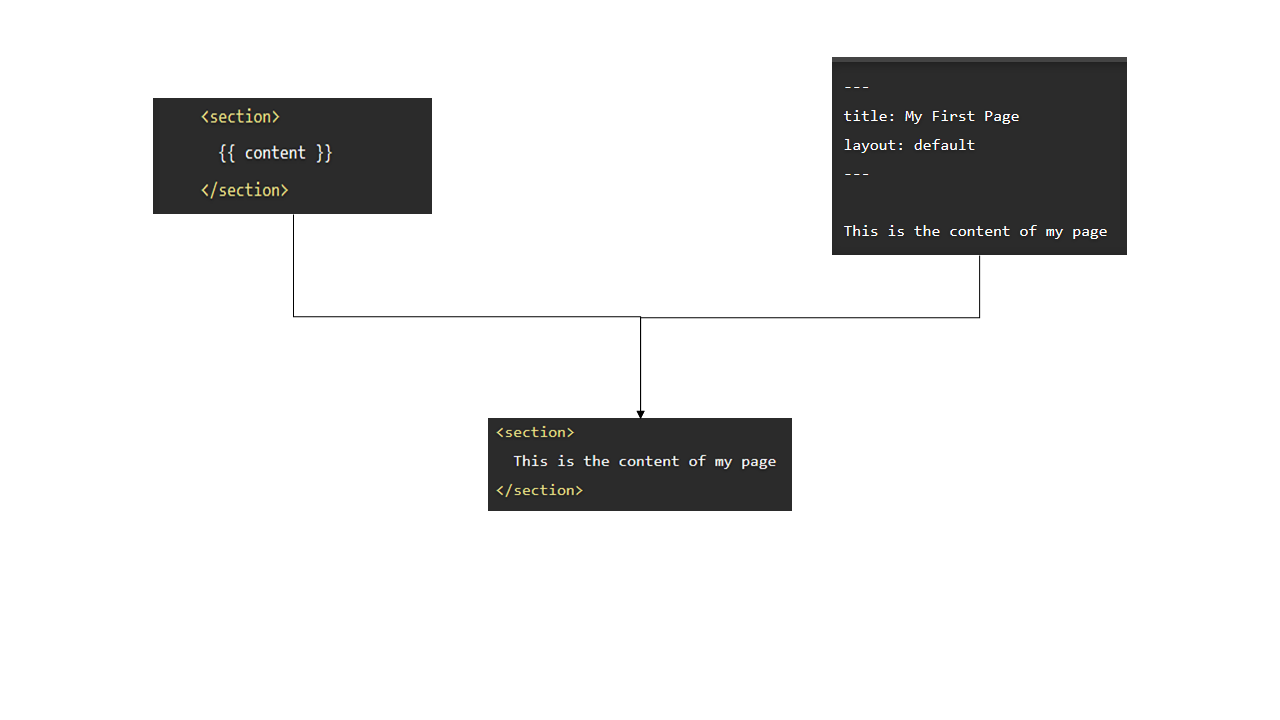
\includegraphics[width=\textwidth]{img/jekyll_process2.png}
    \caption{Proceso de Contenido en Jekyll}
    \label{fig:jekyllProc2}
\end{figure}
\begin{lstlisting}[language=sh]
jekyll new #Crea un proyecto Jekyll
jekyll serve #Construye el sitio web y lo sirve localmente en     
             #"localhost:1400"
jekyll build #Genera el contenido web
\end{lstlisting}
\subsection*{Jekyll en repositorio GitHub}
\label{subsec:jekandGit}
Ya tenemos nuestro servidor mediante el servicio \emph{GitHub Pages}, y para el contenido \emph{Jekyll}, pero ¿Cómo actualizamos nuestra web?¿Cada vez que creamos contenido es necesario actualizar repositorio y ejecutar \emph{Jekyll} por separado?. \\
\emph{GitHub} funciona con Jekyll, lo que quiere decir que cuando creamos contenido y este lo comprometemos (committed), \emph{Jekyll} se encargaŕa de generar el contenido tal y como hemos mencionado.

%%%%%%%%%%%%%%%%%%%%%%%%%%%%%%%%%%%%%%%%%%%%%%%%%%%%%%%%%%%%%%%%%%%%%%%%%%%%%%%
% DUDAS
%%%%%%%%%%%%%%%%%%%%%%%%%%%%%%%%%%%%%%%%%%%%%%%%%%%%%%%%%%%%%%%%%%%%%%%%%%%%%%%
\chapter*{Dudas}
\begin{enumerate}
    \item ¿Por qué los warning de etiquetar?
    \item A la hora de crear los pie de código, hay un problema y es que no permite tener título y pie de foto a la vez, por tanto, ¿dejo el título o dejo el pie de foto?.
\end{enumerate}

%%%%%%%%%%%%%%%%%%%%%%%%%%%%%%%%%%%%%%%%%%%%%%%%%%%%%%%%%%%%%%%%%%%%%%%%%%%%%%%
% SUGERENCIAS TUTOR
%%%%%%%%%%%%%%%%%%%%%%%%%%%%%%%%%%%%%%%%%%%%%%%%%%%%%%%%%%%%%%%%%%%%%%%%%%%%%%%
\chapter*{Sugerencias Tutor}
\begin{enumerate}
    \item 
\end{enumerate}

%%%%%%%%%%%%%%%%%%%%%%%%%%%%%%%%%%%%%%%%%%%%%%%%%%%%%%%%%%%%%%%%%%%%%%%%%%%%%%%
% NOTAS
%%%%%%%%%%%%%%%%%%%%%%%%%%%%%%%%%%%%%%%%%%%%%%%%%%%%%%%%%%%%%%%%%%%%%%%%%%%%%%%
\chapter*{Notas para modificar en la memoria}
\begin{enumerate}
    \item Liquid lo trato en una sección y MarkDown con poco al igual que HTML
    \item ==========================================================
    \item Empezar introducción con una frase del que creo el software Libre
    \item Resumen al principio (Se hace al acabar el proyecto)
    \item Crear estilo para Front Matter
    \item Hablar de gh-pages y de ruby bundle
    \item Gestión de proyecto de Python -> Cap 3 (Cuando acabe el 2)
    \item Para cuando incluimos código, cambiar el tipo de fuente, de manera que haya una para el documento y otra para la parte de incluir código
\end{enumerate}


\end{document}
